\section{簡介}

\begin{frame}{運動紀錄軟體}
\begin{itemize}
\only<1>{
\item 紀錄騎了什麼路線\\
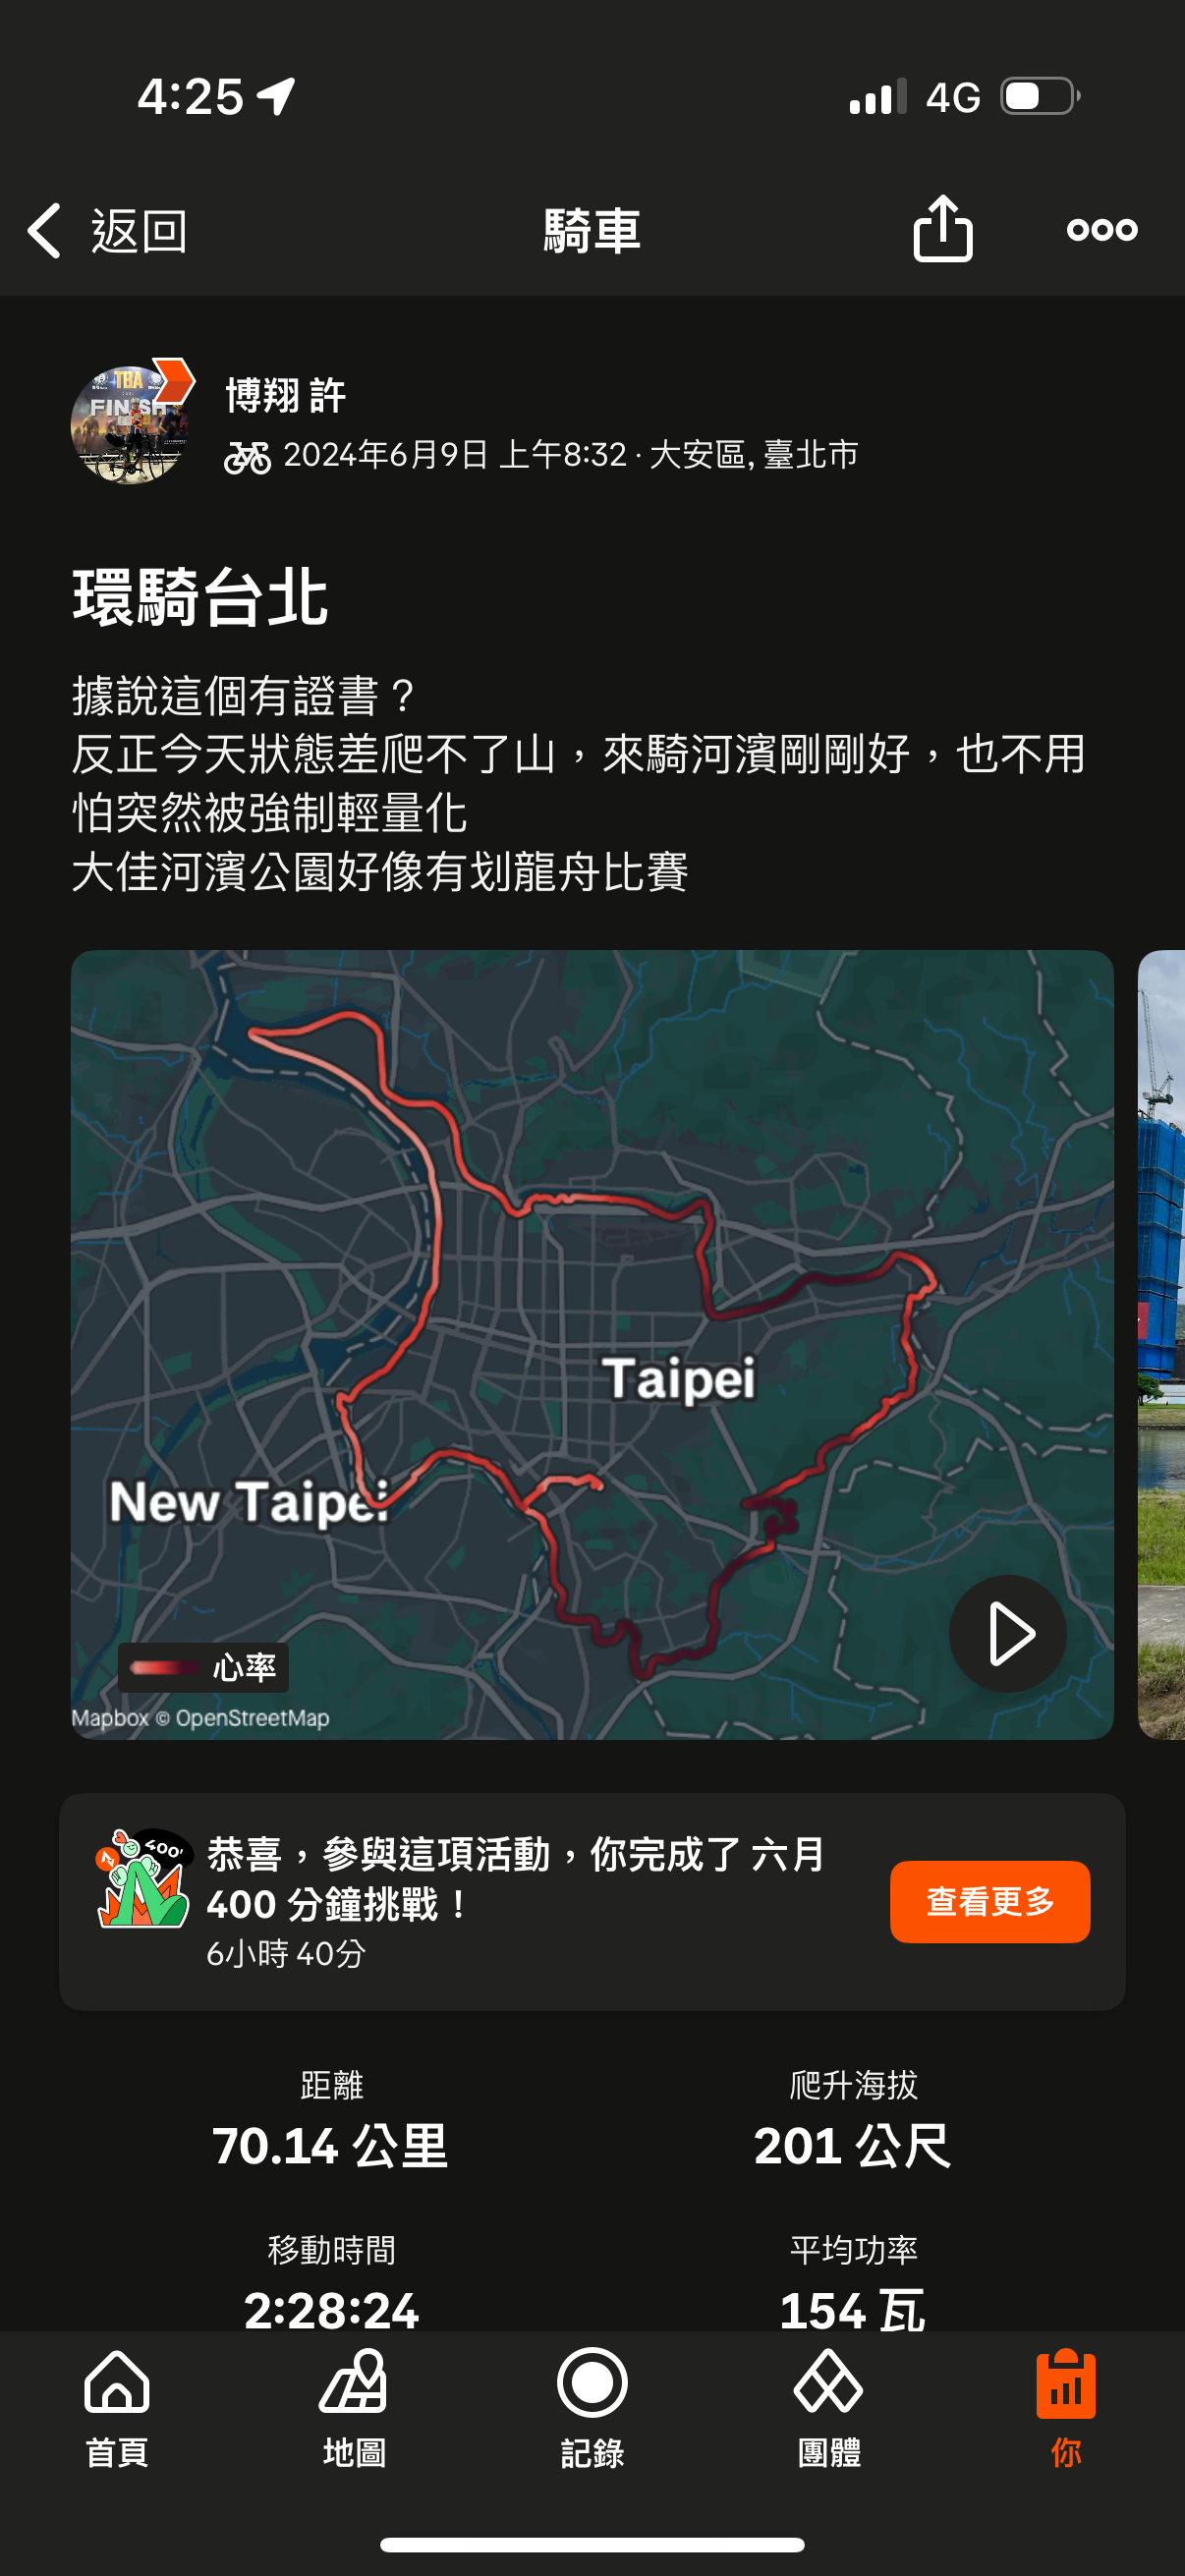
\includegraphics[width=3cm]{smallTaipei.png}
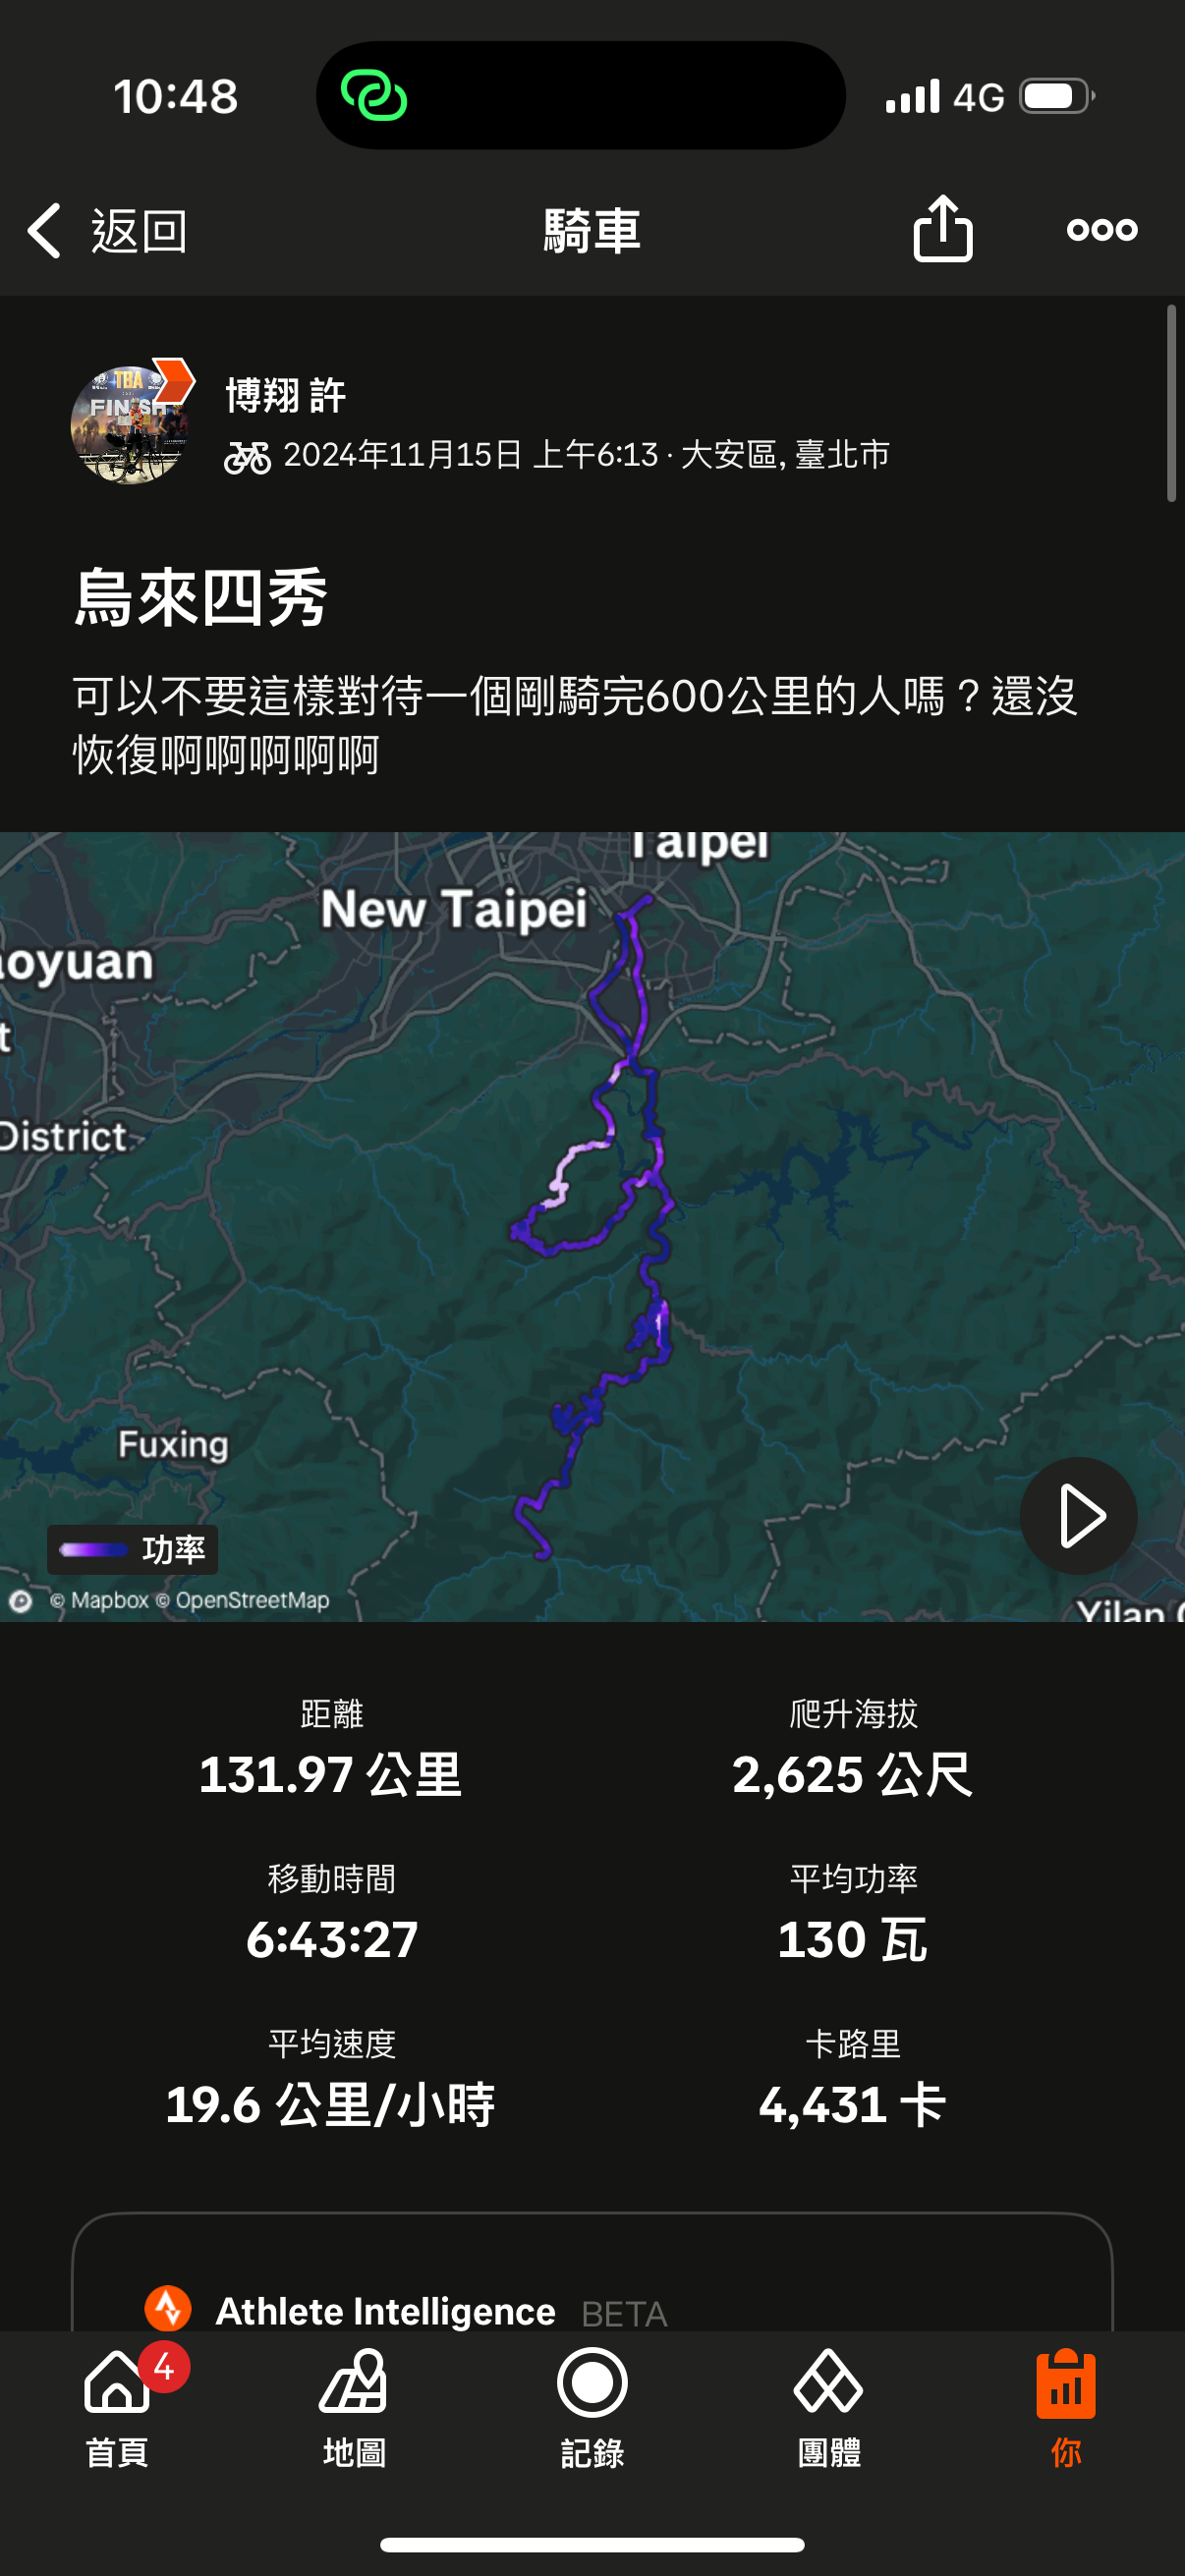
\includegraphics[width=3cm]{wulai4p.png}
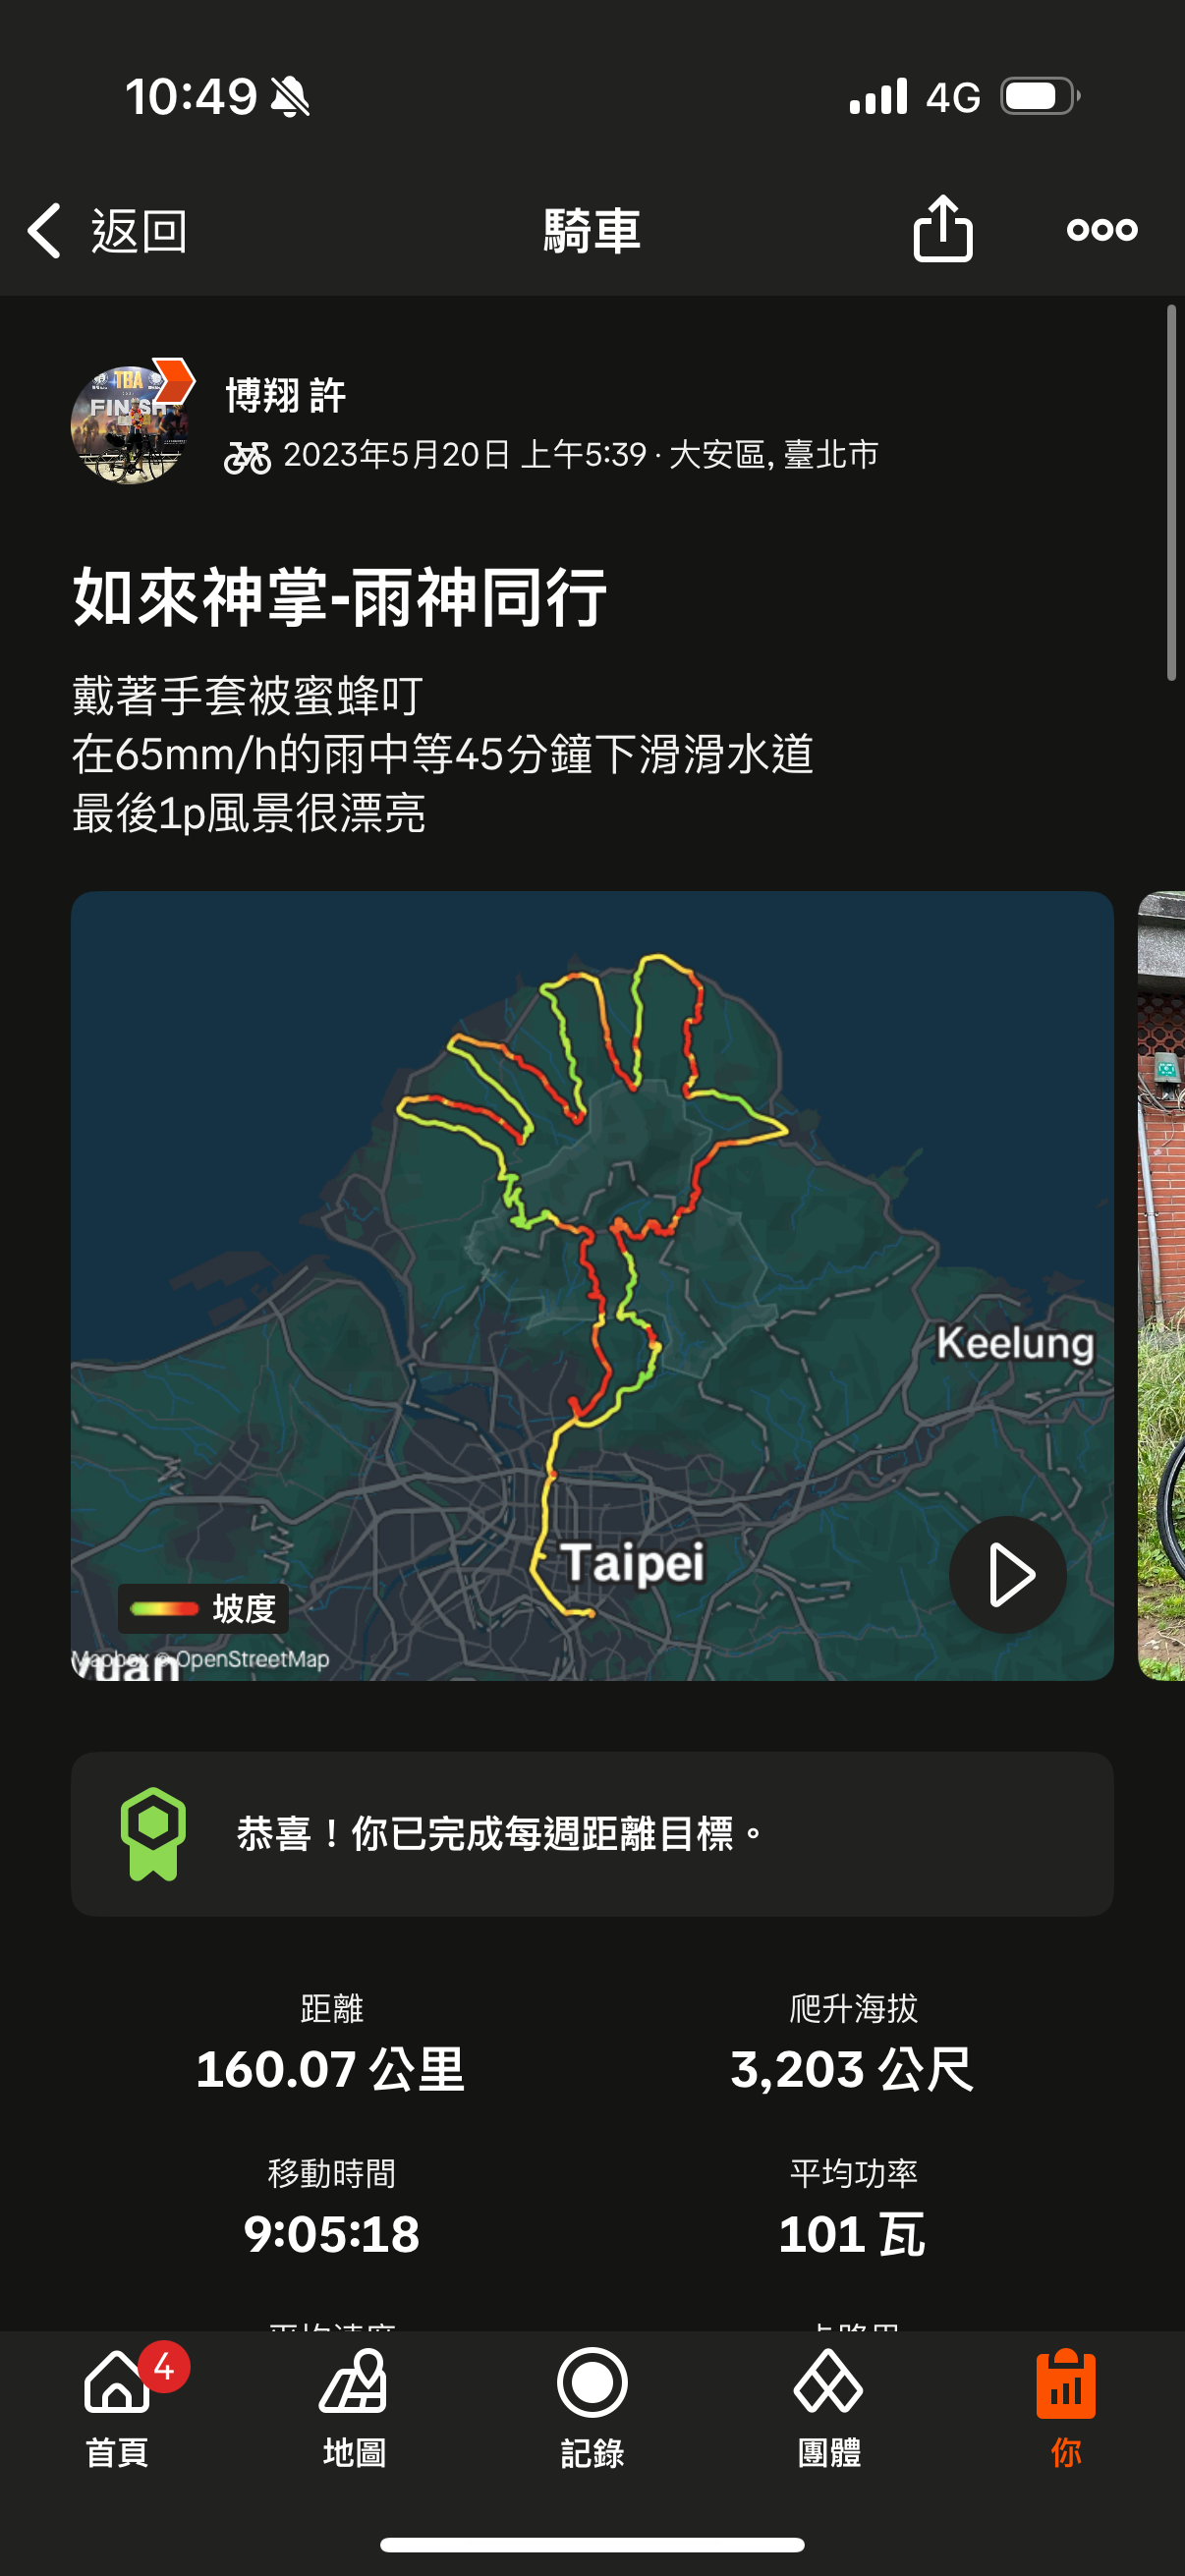
\includegraphics[width=3cm]{hand.png}
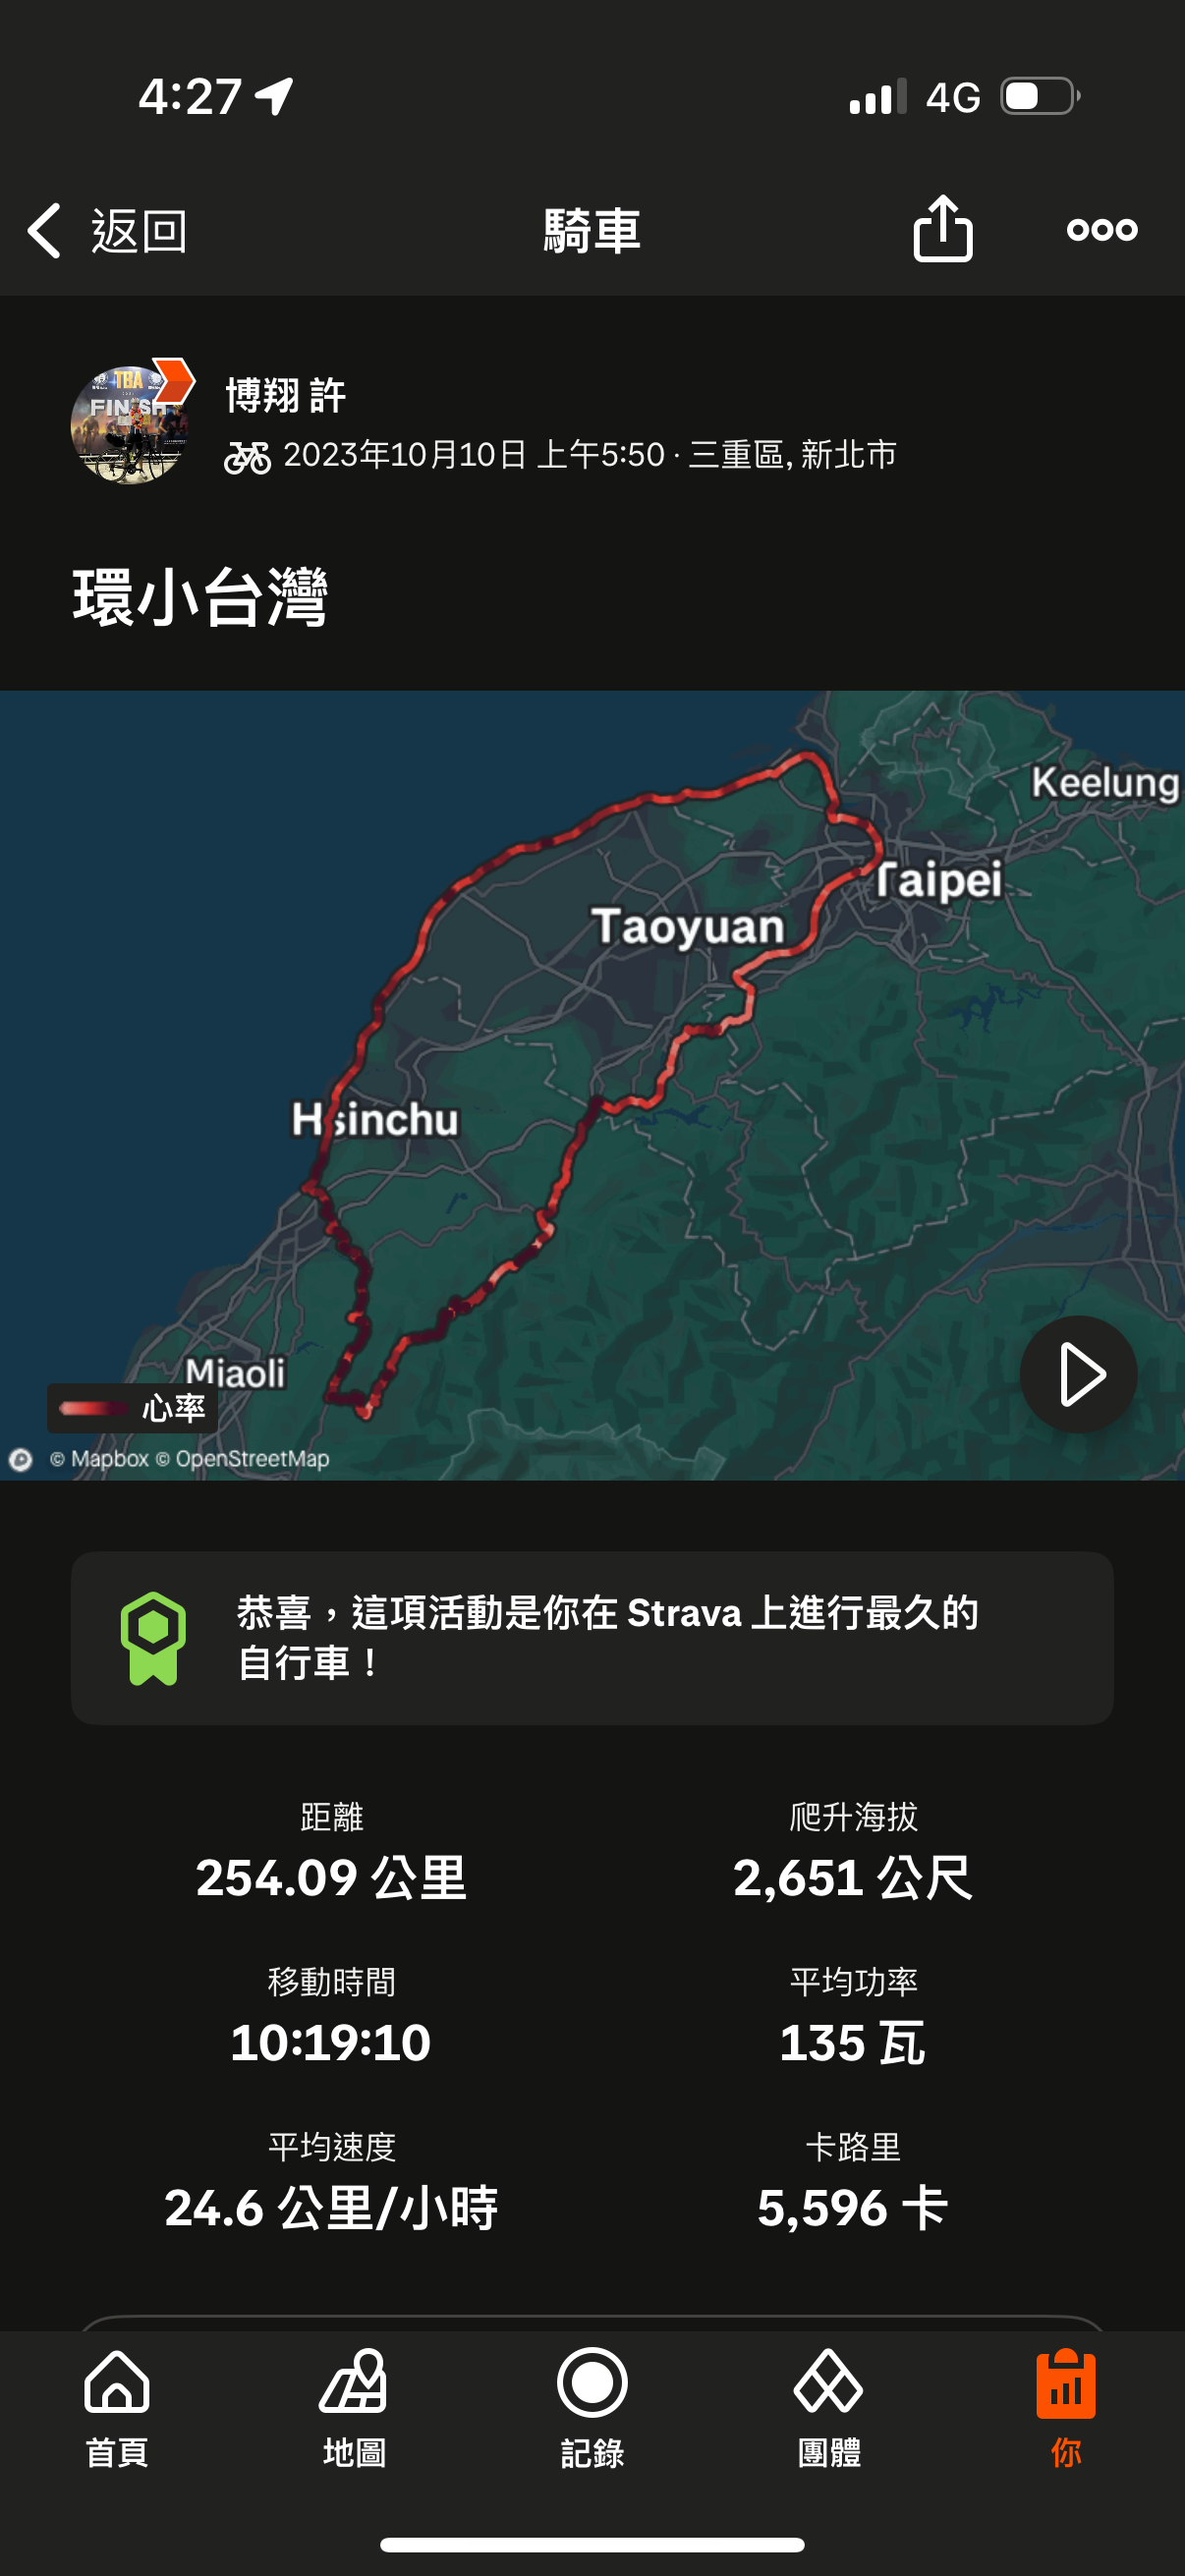
\includegraphics[width=3cm]{smallTaiwan.png}
%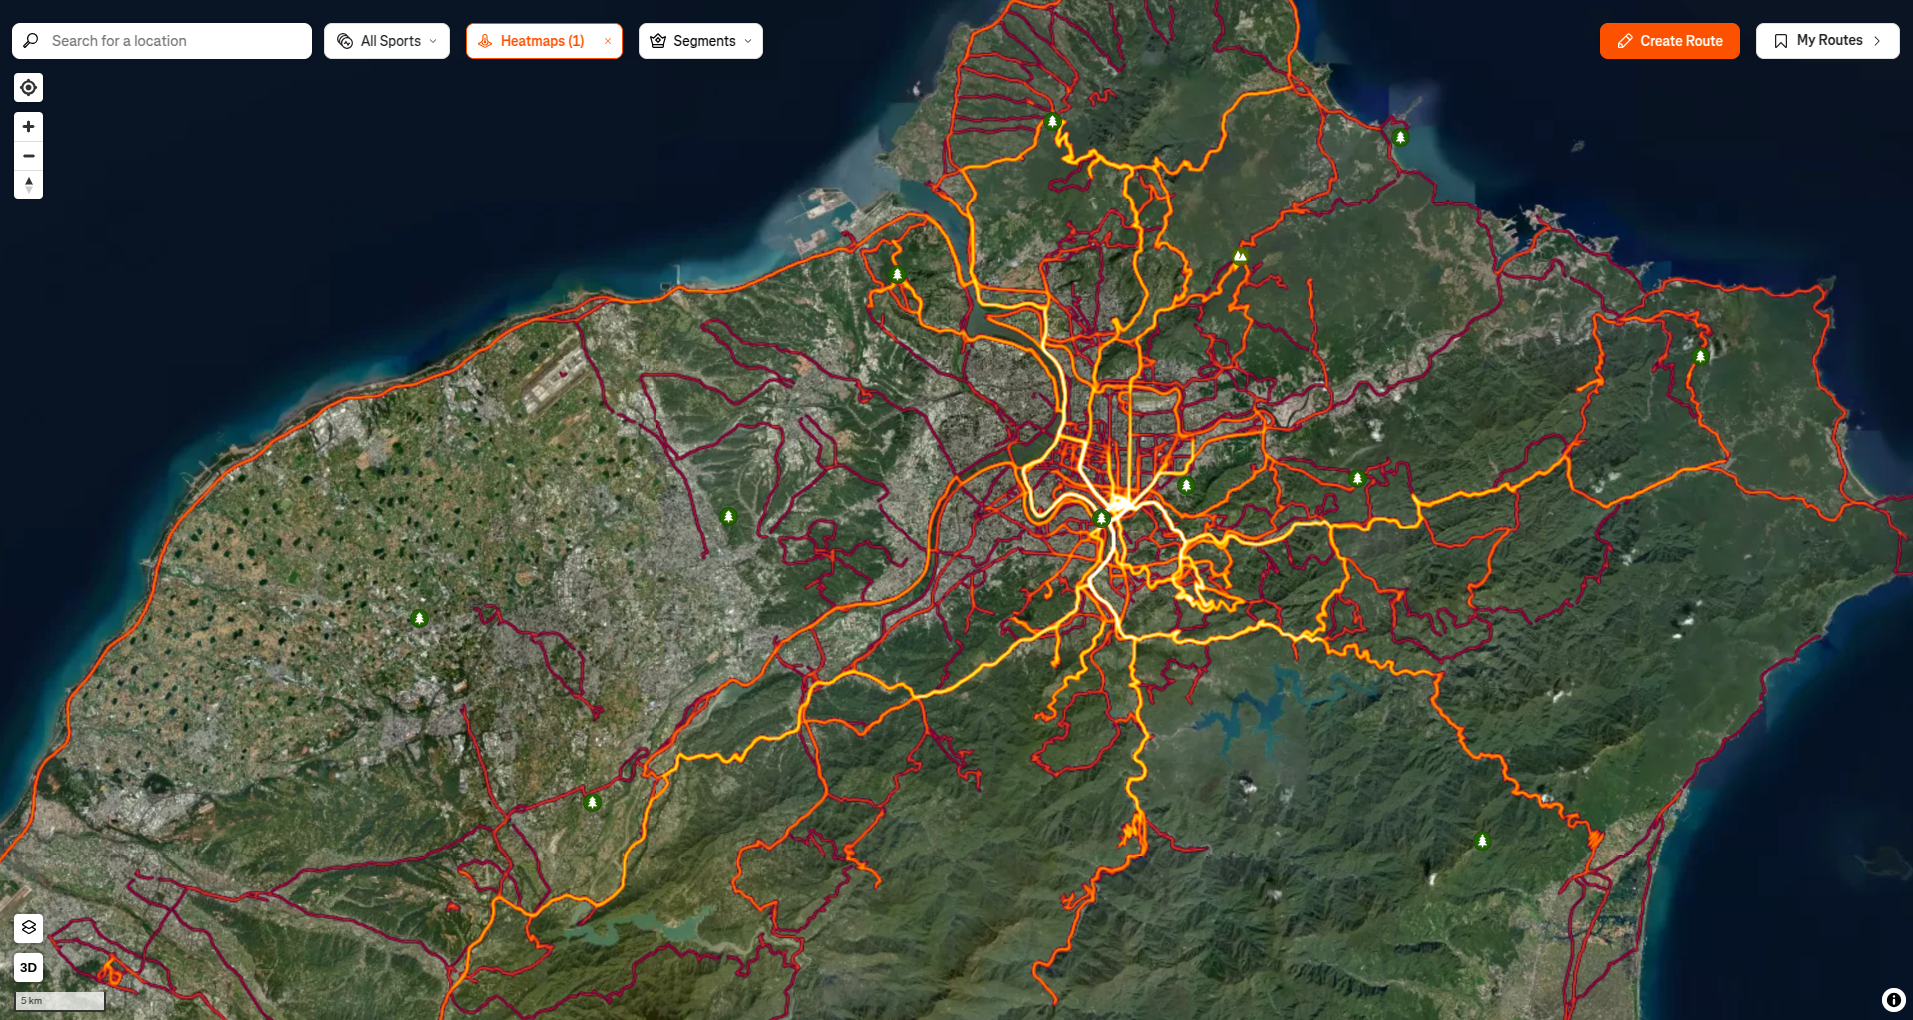
\includegraphics[width=7cm]{taipeiHeatmap.png}
%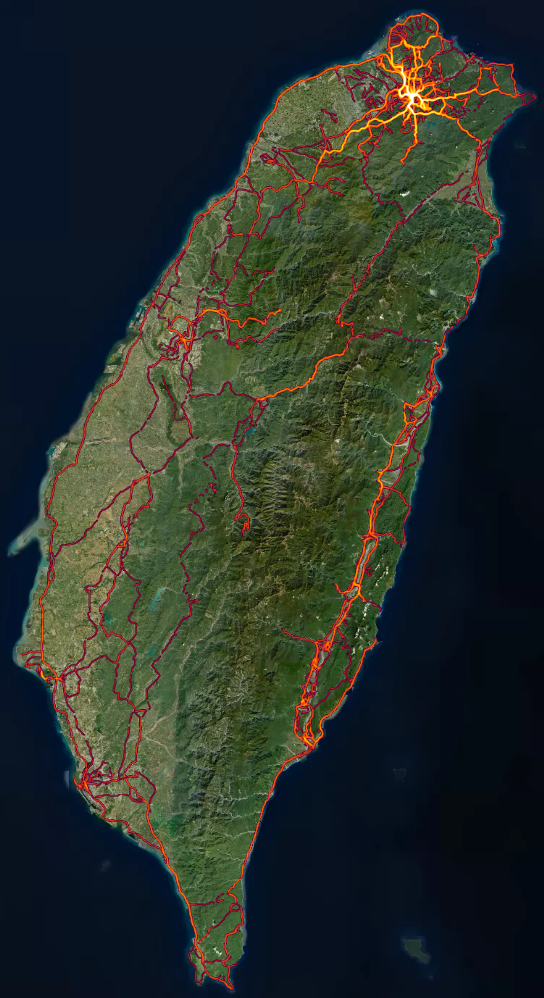
\includegraphics[width=5cm]{taiwanHeatmap.png}
}\only<2>{
\begin{multicols}{2}
\item 統計里程、爬升海拔
\item 分析騎乘的數據(速度、心率、功率等)
\item 看別人騎了什麼路線
\item 跟朋友在同個路段上競速

\includegraphics[width=3cm]{statistics2024.png}
\newpage
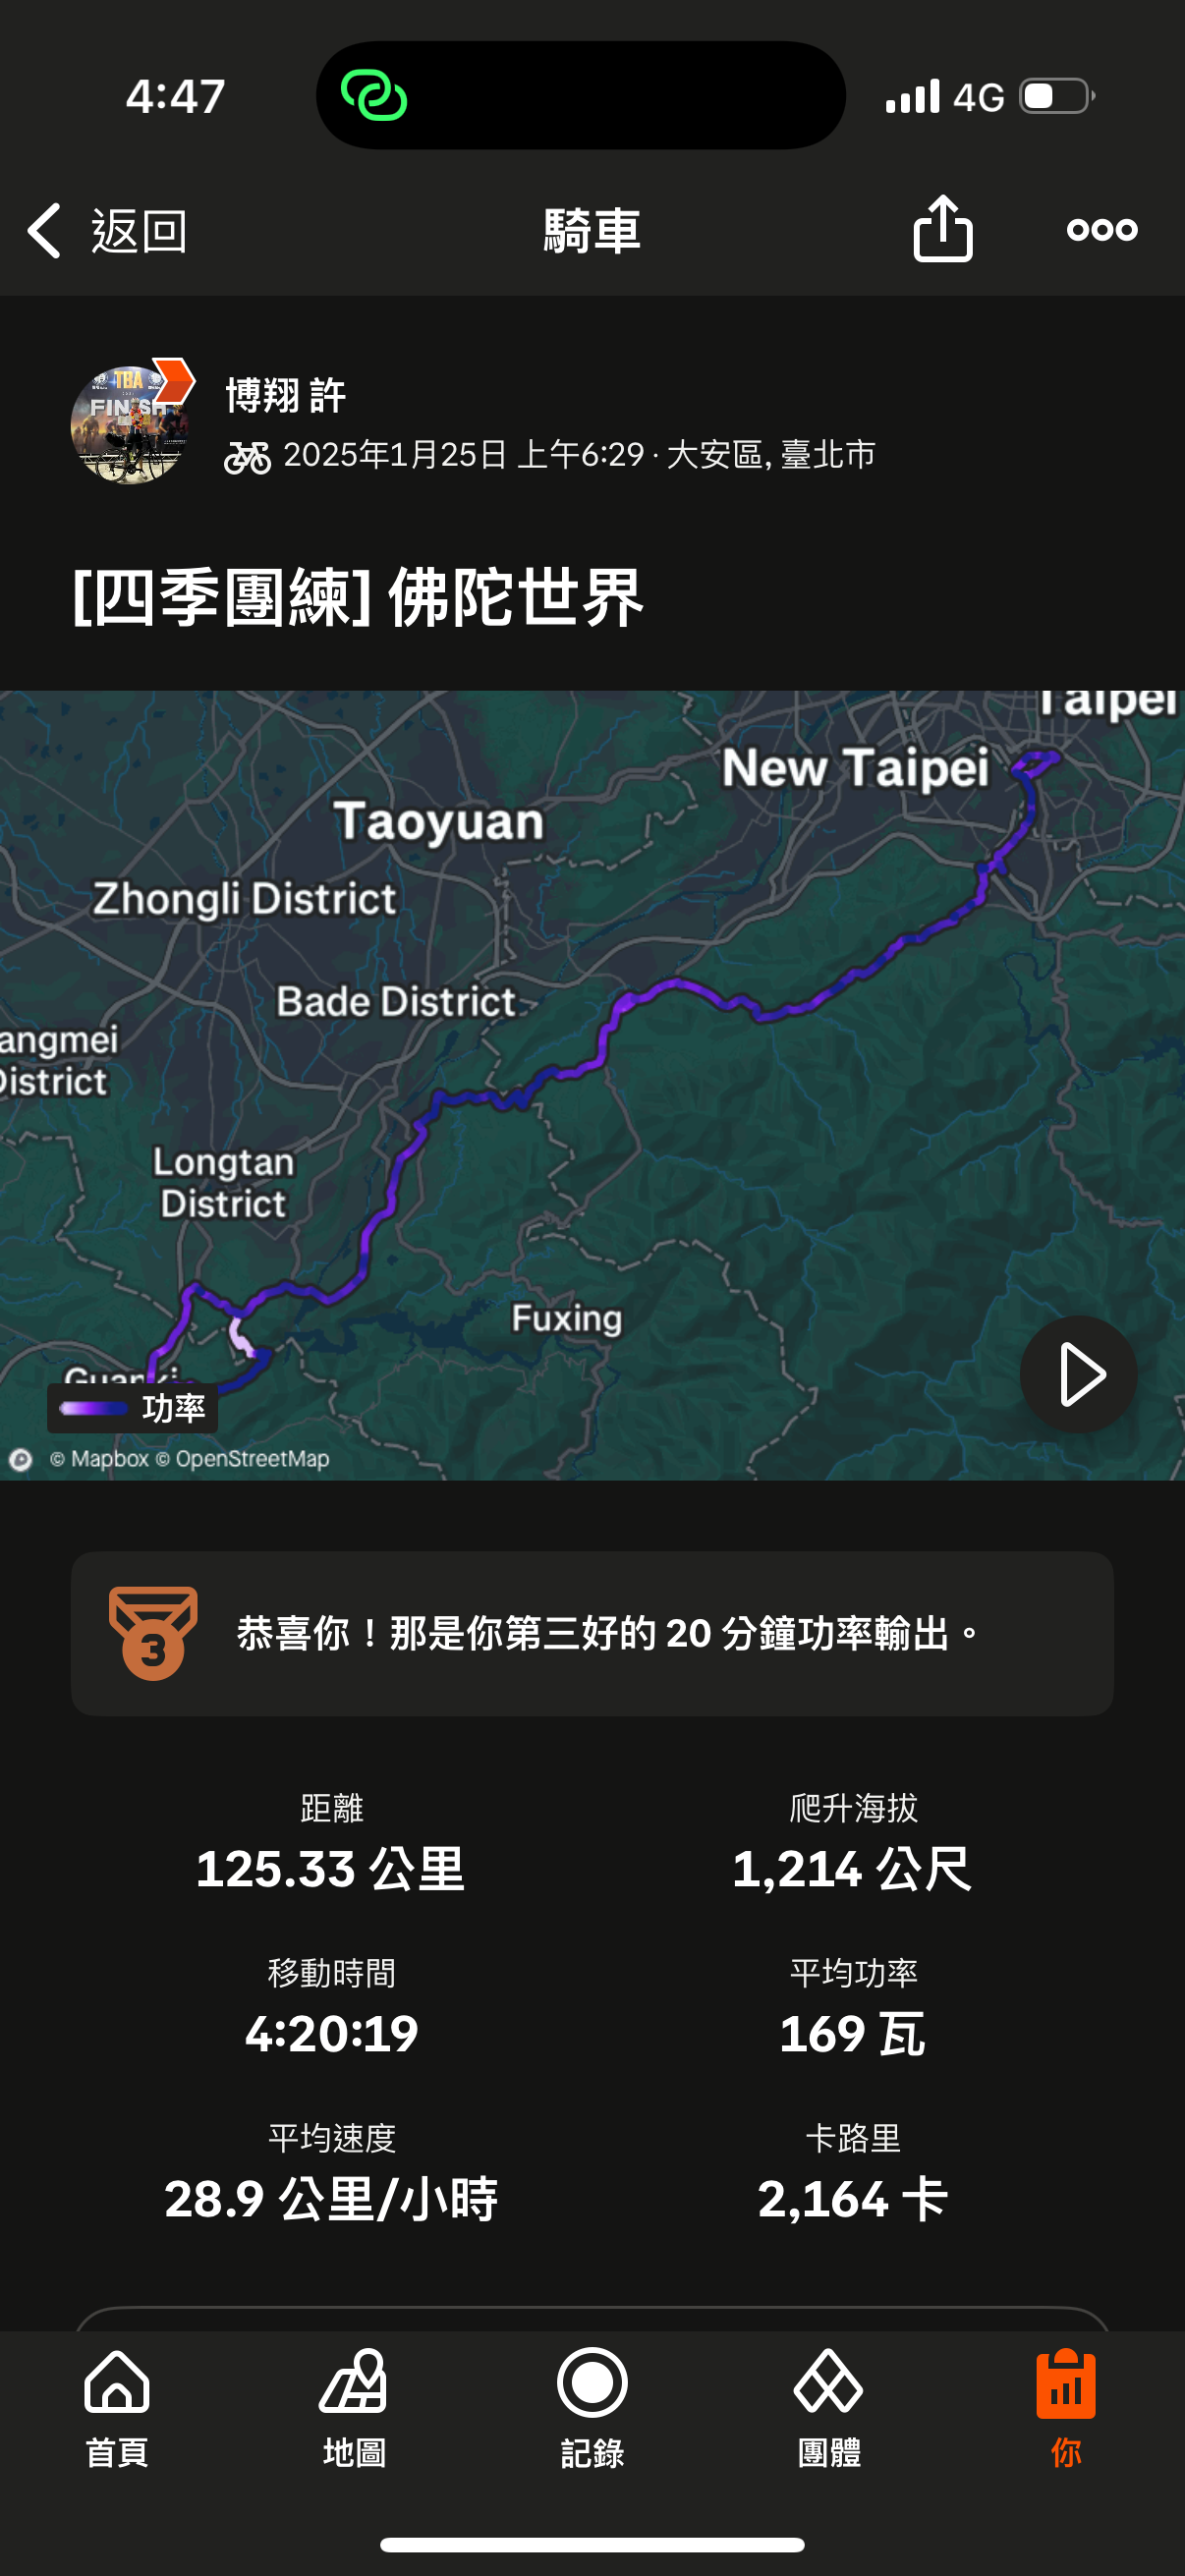
\includegraphics[width=3cm]{photoworld.png}
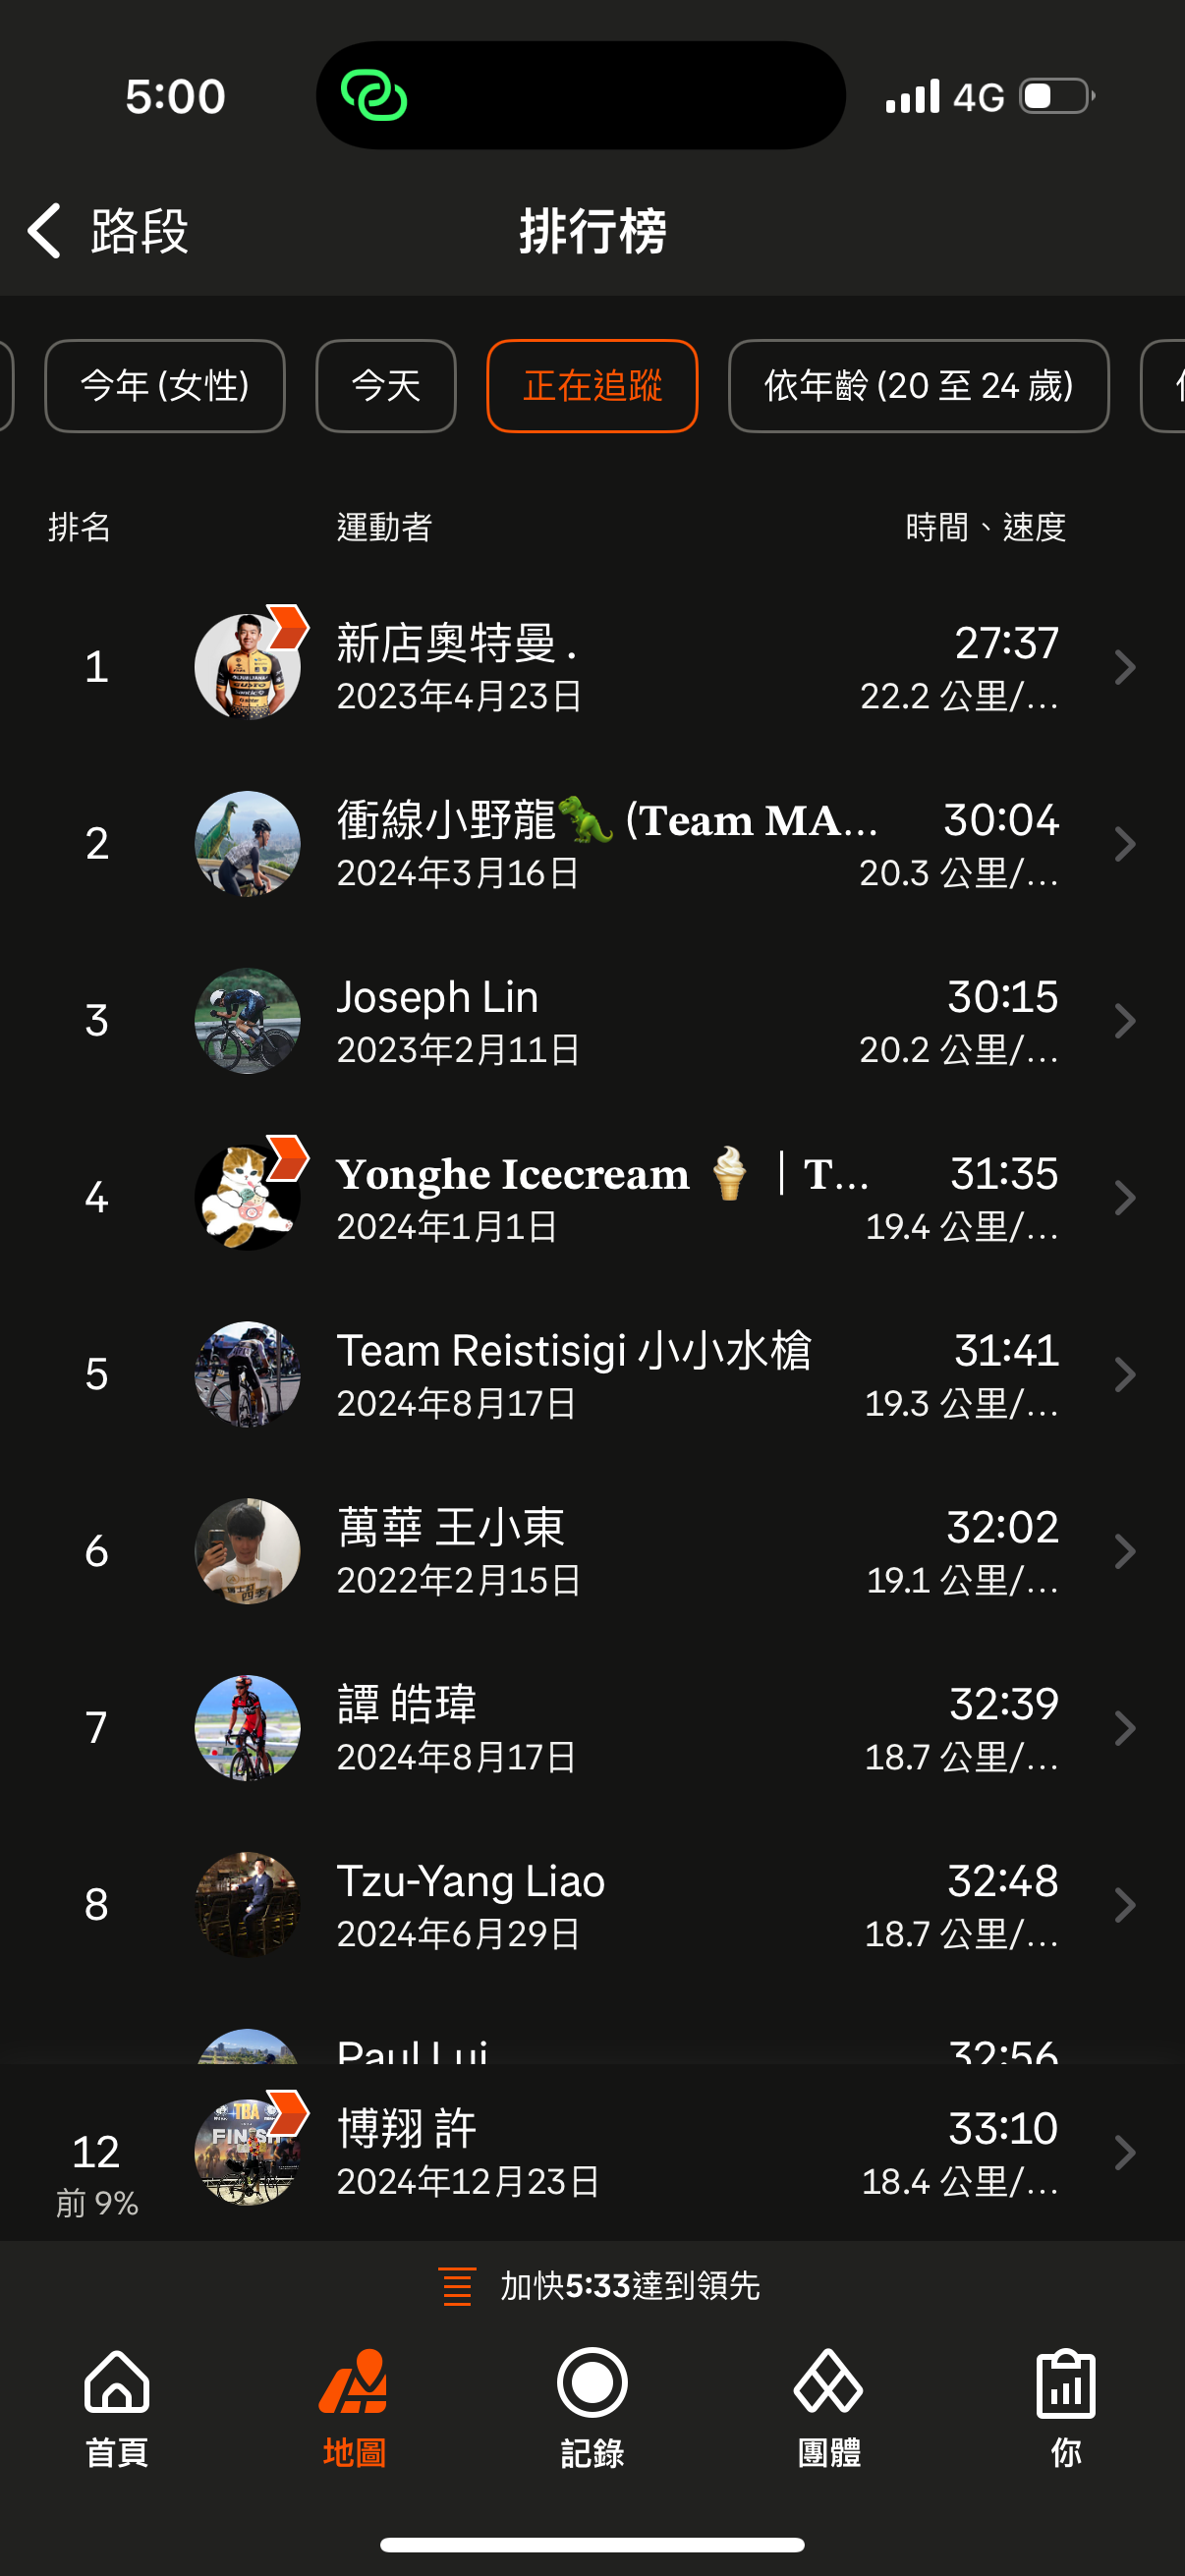
\includegraphics[width=3cm]{balakaRank.png}
\end{multicols}
}
\end{itemize}
\end{frame}

\begin{frame}{常見的運動紀錄軟體}
\begin{itemize}
\item Strava
\item Nike Run Club
\item Garmin
\item Pacer
\item Adidas Running
\item Ride with GPS
\item StepsApp
\item Walkr
\item JoiiSports
\end{itemize}
\end{frame}

\begin{frame}{Strava}
\begin{multicols}{2}
\begin{itemize}
\item 網頁:\url{https://www.strava.com}\\
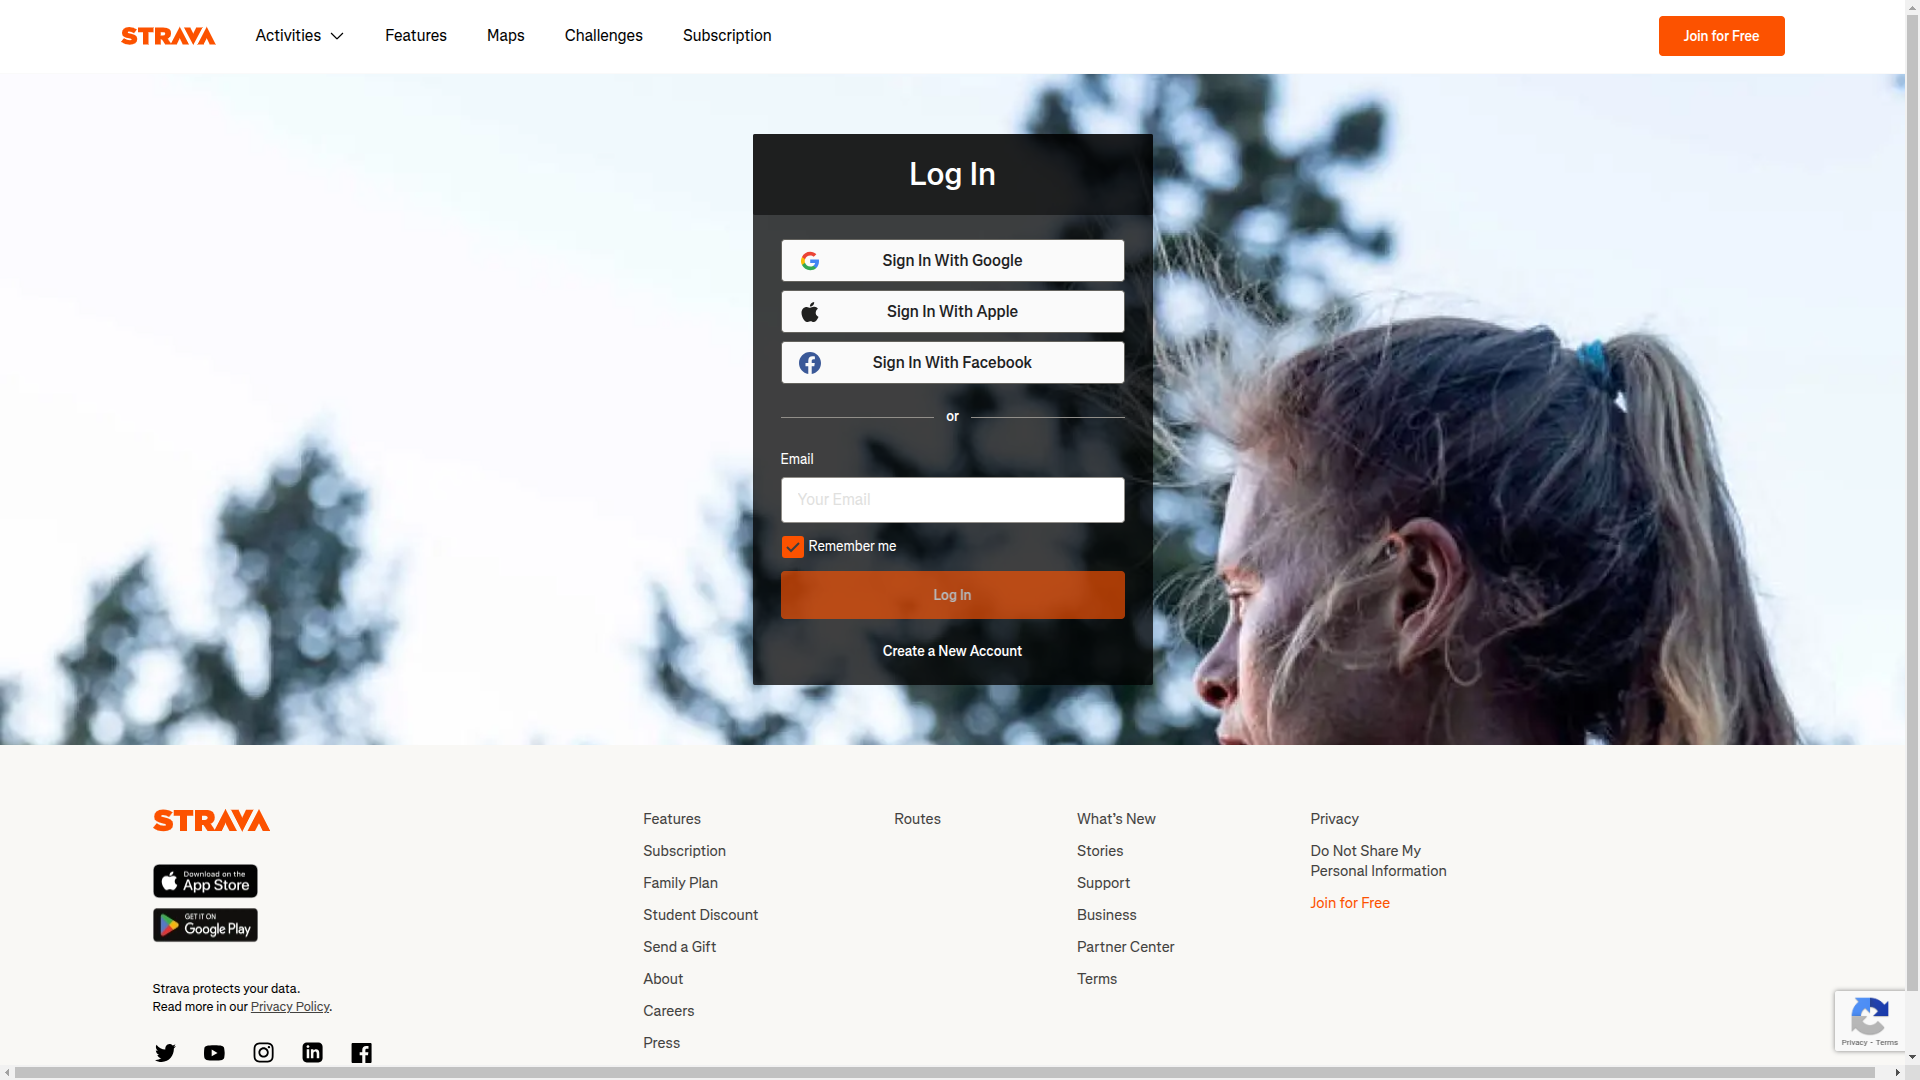
\includegraphics[width=5cm]{stravaWebsite.png}\\

\includegraphics[width=3cm]{rickroll.png}

\includegraphics[width=3cm]{QRcodeStrava.png}
\newpage
\item App:搜尋「Strava」應該就會出現了\\
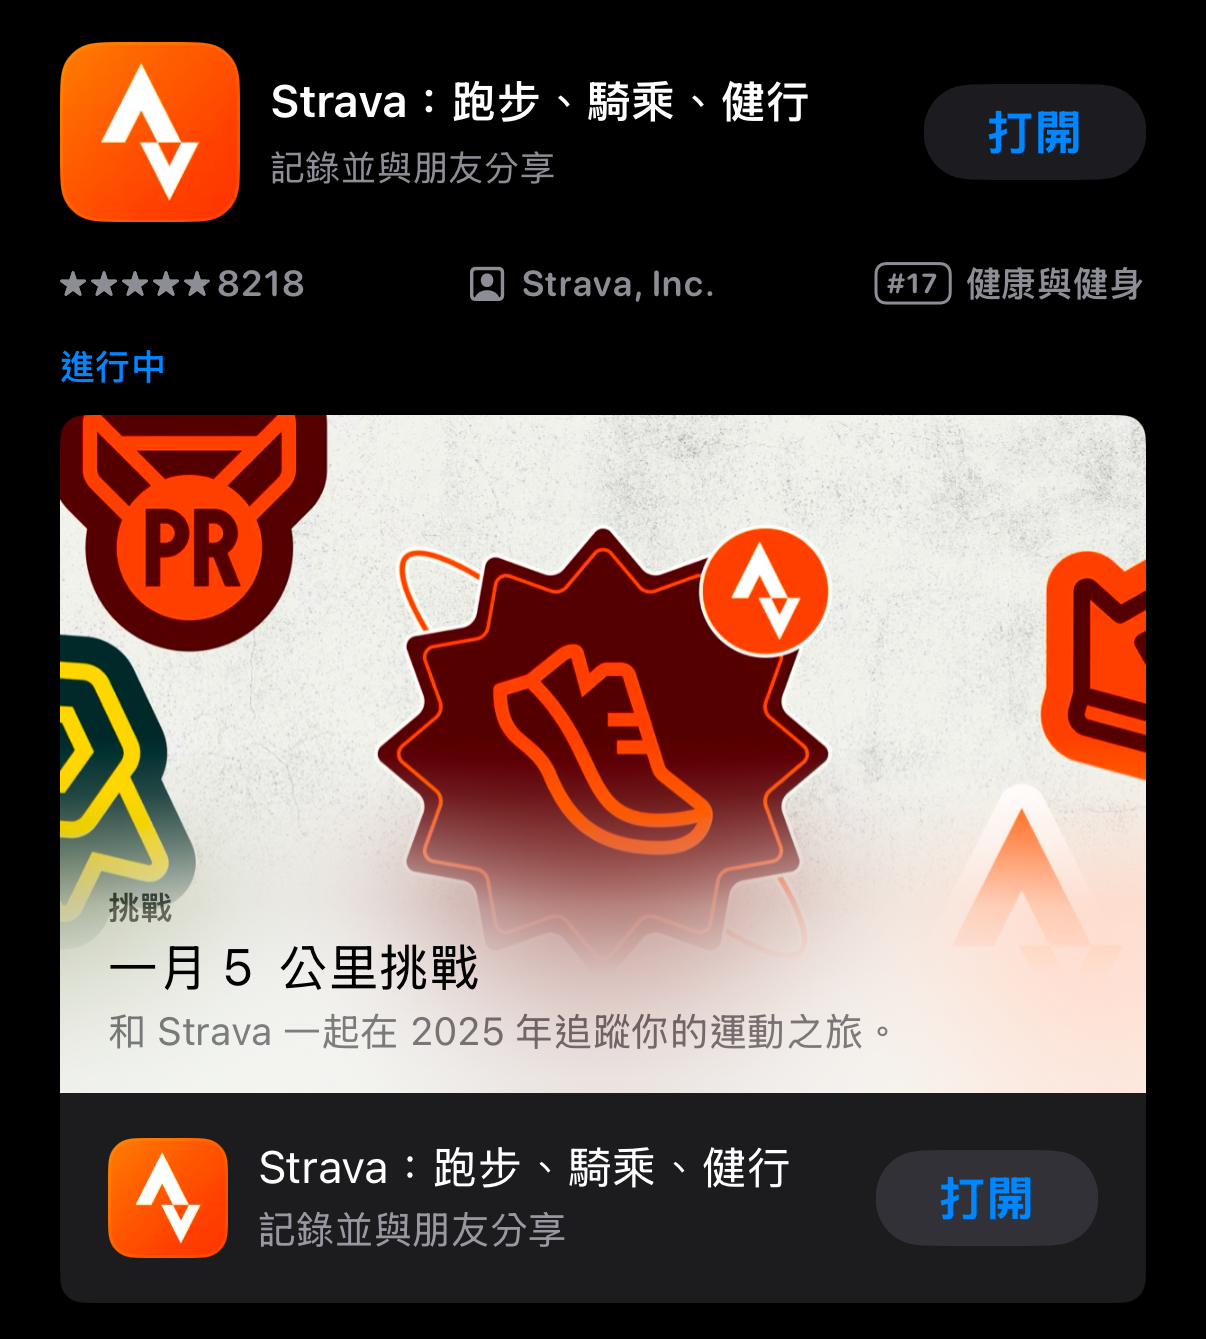
\includegraphics[width=5cm]{stravaApp.png}
\end{itemize}
\end{multicols}
\end{frame}
